\documentclass[11pt, oneside]{article}   	% use "amsart" instead of "article" for AMSLaTeX format
\usepackage{geometry}                		% See geometry.pdf to learn the layout options. There are lots.
\geometry{letterpaper}           
\usepackage[parfill]{parskip} 
\usepackage{graphicx}	
\usepackage{amssymb}
\usepackage{amsfonts}
\usepackage{amsmath}
\usepackage[latin1]{inputenc}
\usepackage{float}
\renewcommand{\abstractname}{}

%\newcommand*{\R}{\mathbb{R}}
%\newcommand*{\abs}[1]{{\lvert#1\rvert}}
%\newcommand*{\Abs}[1]{{\Big\lvert#1\Big\rvert}}
%\newcommand*{\ABS}[1]{{\left\lvert#1\right\rvert}}
%\newcommand*{\set}[2]{{\{#1 \mid #2\}}}
\def\i{\hat{\imath}}
\def\dt{\Delta t}
\def\dtm{\Delta t_{\mathrm{max}}}
\def\tc{\tau_{\mathrm{crunch}}}

\title{Gravitational $N$-Body Simulations}
\author{Gudbrand Tandberg}
\date{\today}							% Activate to display a given date or no date

\begin{document}
%====================MAIN PAPER==============================
\maketitle

%====================Section 1==============================

\begin{abstract}
In this article we will study the numerical modelling of gravitationally interacting $N$-body systems. The first part of the article focuses on introducing the subject matter and presenting some of the results of the early simulations. The numerical methods are first explained and then tested on the simple model consisting of the inner solar system. We then proceed to present a upgraded version of the solver featuring adaptive timesteps and parallellization. The simulations of the inner solar system are re-run and compared with the ones previously obtained. In the second part of the article we turn our attention to increasing $N$. We use as our physical system that of a uniform spherical distribution of point-masses at rest. This system is meant to model a small cluster of stars. We study some of the physics of such a system and also consider some numerical aspects of increasing $N$. All the programs, animations and articles referred to in the paper can be found at http://github.com/gudbtandberg/N-Body.
\end{abstract}

\section*{Foreword}

This article is the final project in the course \emph{FYS3150 - Computational Physics} at the University of Oslo autumn 2014.

\section{Introduction to the $N$-body problem}

We start off by giving the basic definition of the problem to be solved. The system consists of $N$ point-masses moving in space under the influence of mutual gravitational forces. Denote the mass, position and velocity of body $i$ as $m_i, r_i$ and $v_i$ respectively (the latter two being three dimensional vectors). According to Newton, the gravitational acceleration on body $i$ is given by

\begin{equation}
a_i = \sum_{j\neq i}\frac{Gm_j}{r_{ij}^2}\i_{ij},
\label{gravity}
\end{equation}

where $r_{ij}$ is the distance between body $i$ and $j$, $G$ is the gravitational constant and $\i_{ij}$ is the unit vector pointing from body $i$ towards body $j$. This can be used to determine the differential equations of motion for all the particles by decoupling Newton's second law as a system of ordinary first order differential equations as follows

\begin{equation}
\begin{bmatrix}
r_i \\
v_i \\
\end{bmatrix}'
= 
\begin{bmatrix}
v_i�\\
a_i \\
\end{bmatrix}.
\label{diffeq}
\end{equation}

From now on we refer to the couple $(r, v)$ as the \emph{state} of a body. All in all this gives us one 6-dimensional coupled ordinary differential equation for each body, or $6N$ ordinary differential equations. All that is needed to simulate such a system for any discretized period of time $T$ is the initial positions and velocities of all of the bodies along with a rule for how to move the system from one time to the next. Such rules will be discussed further in the next section.

\subsection{Scaling the equations}

In the problem set forth in the previous section we saw that there were three different units of measurement; length, time and mass. To simplify the numbers involved in a simulation, the equations should be scaled appropriately. In the case of the solar system, the natural unit of length is the astronomical unit, defined to be the mean distance between the Sun and the Earth; approximately $1.49\cdot 10^{11}$ m. We arbitrarily choose one week as our unit of time, or $60\cdot60\cdot24\cdot7$ s. We could fix the unit of mass to be the mass of the Earth or Sun, but instead choose the mass scale so as to fix $G = 1$. This is equivalent to fixing the unit of mass. In scaling the equations, what we are really doing is performing the change of variables

\begin{eqnarray}
r \to \frac{r}{r^*} \\
t \to \frac{t}{t^*} \\
m \to \frac{m}{m^*} \\
\end{eqnarray}

where $r^*, t^*$ and $m^*$ are the characteristic lengths of the units involved. To find out what our characteristic mass will be, we first note that the unscaled value of $G$ in SI-units is $G = 6.67\cdot10^{-11} \mathrm{m}^3/\mathrm{kg}\cdot\mathrm{s}^2$. Denoting the scaled value of $G$ by $G^*$, we get that

\begin{equation}
G^* = \frac{6.67\cdot10^{-11} \mathrm{m}^3/\mathrm{kg}\cdot\mathrm{s}^2\cdot m^*\cdot{t^*}^2}{{r^*}^3}
\label{scaleG}
\end{equation}

Setting this equal to one and solving for $m^*$ yields

\[
m^* = \frac{{r^*}^3}{6.67\cdot10^{-11}\mathrm{m}^3/\mathrm{kg}\cdot\mathrm{s}^2 {t^*}^2}
\]

In our case

\begin{equation}
m^* = \frac{\mathrm{AU}^3}{6.67\cdot10^{-11}\mathrm{m}^3/\mathrm{kg}\cdot\mathrm{s}^2\cdot\mathrm{week}^2} = 1.371\cdot10^{32}  \mathrm{kg}
\end{equation}

or roughly one hundred solar masses. The only point in the program where the units come into the picture are in the setting up of the initial conditions. All values in the input files for the inner solar system are in these units. 

\subsection{A brief history the N-Body problem}

For the simple case of $N=2$, closed form analytical solutions to the problem defined by \eqref{gravity} and \eqref{diffeq} exist. In fact, these solutions were first discovered by Newton himself. The idea in his solution consists of a series of simplifications; first eliminating some unknowns by changing coordinates to the centre of mass coordinates, then using conservation of angular momentum to assert that all the motion will be in a plane to eliminate 4 more unknowns. Finally, the trajectories of the bodies can be shown to follow conic sections. This result is consistent with Kepler's earlier discovery that bound planets move in ellipses, and unbound bodies move in hyperbolic or parabolic trajectories. This must have motivated Newton to take on the three-body system, which he did in his lunar investigations in Principia. But no general solutions were found. 

Finding analytical solutions of the three-body problem stood unsolved for over two centuries until Poincar� showed that there is no general closed form solution to the three-body problem. Furthermore it was shown by him that the trajectories are generally non-repeating, or chaotic in modern terms. This must have shocked the scientific community, shattering (not for the last time) any idea of a 'clockwork universe'. 

Poincar�'s discovery did not however halt further research into the three-body problem. Further contributions to the problem were put forward by Lagrange, Liouville, Laplace, Jacobi, Darboux and Hamilton amongst others. It was discovered that in many special cases closed form solutions do exist. At the time of writing 16 families of solutions to the three-body problem are known. 13 of these were discovered in 2013.

With the advent of computers in the middle of the 20th century, the $N$-body problem could finally be studied in further detail for $N > 3$. As computing power increased exponentially, larger and larger systems could be studied. Today, large $N$ simulations are used as tools in astrophysics and cosmology to study concepts such as the evolution of star clusters, or even the evolution of the large scale structure of the universe. A modern example of such a simulation is the so-called Millennium Run, where the trajectories of $2160^3$ (just over 10 billion) bodies were computed. The computation lasted over a month on a super computer in Switzerland. 

\section{The numerical methods}

In this section we present the two different methods used to move the bodies forward in time, so-called integration schemes. The two methods we will use are the Velocity Verlet method and the fourth order Runge Kutta method. We assume we are at a time $t$, where the quantities $r(t)$ and $v(t)$ are known, and we wish to determine $r(t+\dt)$ and $v(t+\dt)$. In the following derivations we only consider the state of one body and adopt the notation $r_i = r(i\dt), v_i = v(i\dt)$, where $i = 1, \cdots, n$ and $\dt$ is the time step. 

\subsection{The Velocity Verlet method}

The first integration method we utilise in our simulations is the \emph{Velocity Verlet} method. It is characterised by the equations

\begin{eqnarray}
v_{i+1/2} = v_i + a_i\dt /2\\
r_{i+1} = r_i + \dt v_{i+1/2}\\
v_{i+1} = v_i + \dt\frac{a_i + a_{i+1}}{2}
\end{eqnarray}

First we compute a better approximation to the velocity at time $i$ by using the computed value $v_{i+1/2}$. This will be recognised as the Taylor expansion of the velocity at time $i$ truncated to second order. This value is then used to compute the position at time $i+1$. To compute the value of the velocity at time $i+1$ the acceleration at time $i+1$ is first computed using the newly found positions at time $i+1$. The velocity is then set to the current velocity plus the time step times the average acceleration between time $i$ and time $i+1$. We note that only one force evaluation is necessary at each step, since the acceleration $a_{i+1}$ found at any time can be stored and used as $a_i$ in the next step. We do not derive the order of the error terms, but simply state the fact that the local error (the error that occurs when stepping from one time step to the next) is of order $\mathcal{O}(\dt^4)$ in position, but only of order $\mathcal{O}(\dt^2)$ in velocity. The global error (the accumulated error after many timesteps is of order $\mathcal{O}(\dt^3)$. It shall be interesting to observe these facts in the simulations presented later on. 

As an aside we can mention that the Verlet integration scheme has the nice properties of being a sympleptic and time-reversible scheme, meaning that it conserves the energy of the system well, and it can be run backward and return exactly to a earlier initial condition. These are for obvious reasons desirable properties when solving the $N$-body problem.

\subsection{Runge Kutta 4}

The second method we use is the Runge-Kutta fourth order method. For notational purposes we introduce the function

\begin{equation}
f\left(\begin{bmatrix}r \\ v \end{bmatrix}\right) = \begin{bmatrix} v�\\ a�\end{bmatrix} 
\end{equation}

The Runge-Kutta method uses four quantities to get from time $i$ to time $i+1$. These are

\begin{eqnarray}
k_1 = f\left(\begin{bmatrix}r_i \\ v_i \end{bmatrix}\right) \\
k_2 = f\left(\begin{bmatrix}r_i \\ v_i \end{bmatrix} + \frac{\Delta t}{2} k_1\right)\\
k_3 = f\left(\begin{bmatrix}r_i \\ v_i \end{bmatrix} + \frac{\Delta t}{2} k_2\right)\\
k_4 = f\left(\begin{bmatrix}r_i \\ v_i \end{bmatrix} + \Delta t k_3\right)\\
\end{eqnarray}

The step is then taken as

\begin{equation}
\begin{bmatrix}r_{i+1} \\ v_{i+1} \end{bmatrix} = \begin{bmatrix}r_i \\ v_i \end{bmatrix} + \frac{\Delta t}{6}(k_1 + 2k_2 + 2k_3 + k_4)
\end{equation}

The phase space 'tangent' is computed by averaging four computed approximations at three different timesteps, one at the start, one at the end and two in the middle. We see immediately that this is a costly method since at each step it requires four gravity evaluations. However, the accuracy is much greater than the simple Verlet method. In fact, the local error is of order $\mathcal{O}(\Delta t^5)$, while the global error is of order $\mathcal{O}(\Delta t^4)$.

\section{The first NBodySolver class}

In this section we describe the basic behaviour of the first $N$-body solver used in the simulations. The program can be found in \verb+source/NBodySolver.cpp+ in the main project page. The program uses a object-oriented structure, the main objects being \verb+NBodySolver+, and \verb+Body+. The former acts as the controller object. It is initialised as \verb+NBodySolver(N, T, dt, method)+. Methods for initialising, solving and finally writing the results to files are all called from a main program, in our case \verb+main.cpp+. 

The most important attribute of the NBodySolver class is the list of bodies; \verb+bodies+. Each body has attributes \verb+r+ and \verb+v+ corresponding to the position and velocity at the present time. In addition, each body keeps track of the positions and velocities at all previous times in the matrix \verb+state_history+. This matrix is incrementally updated at each pass of the main integration loop.

The integration loop, implemented in the \verb+solve()+-method is the most central part of the program. In pseudocode, the algorithm is as follows

\begin{verbatim}
while global time < T
    extract the states of all the bodies
    step all planets using either Verlet of Runge Kutta
    update positions and velocities of bodies
    global time++
\end{verbatim}

There are of course some technicalities regarding the specific implementations of the different integration methods, but the explanation of these are left to the comments.

After the integration loop is finished, the main program calls the \verb+writeTrajectories()+ and \verb+writeEnergy()+ methods of the solver. As this project features a lot of output a necessarily cumbersome naming convention was adopted for file writing: 

\begin{verbatim}
N_body_type_T_dt_adaptive_method_cpus_eps.dat,
\end{verbatim}

where \verb+type+ is either energy or trajectories, \verb+N, T+ and \verb+dt+ are obvious, \verb+adaptive+ is either 0 or 1, \verb+method+ is either 0 (Verlet) or 1 (RK4), and \verb+cpus+ and \verb+eps+ are the number of cpus to be used and the smoothing factor respectively, to be explained in a later section. 

\section{Results for the solar system}

We now present our results from testing the first $N$-body solver class on the inner solar system. The system consists of the sun and the six innnermost planets of the solar system. We integrate the system for one Giovian year, or roughly 619 weeks. The simulation is run for three different values of $\dt$ for both methods. 

\begin{figure}[H]
\begin{center}
\includegraphics[width=12cm]{./figures/trajectories1}
\caption{Solar system trajectories integrated with the Velocity Verlet method over one Giovian year using three different timesteps}
\label{traj1}
\end{center}
\end{figure}

\begin{figure}[H]
\begin{center}
\includegraphics[width=12cm]{./figures/trajectories2}
\caption{Solar system trajectories integrated with the fourth order Runge-Kutta method over one Giovian year using three different timesteps}
\label{traj2}
\end{center}
\end{figure}

In fig. \ref{traj1} and \ref{traj2} we see the computed trajectories. For both methods we see the thickness of each of the orbits decreases as $\dt$ decreases. This is to be expected, as a smaller timestep increases the accuracy. Even at the smallest timestep, the orbits are somewhat 'smeared' out in space, but this is not necessarily a artifact of poor accuracy, it just so happens that the sun also moves along in space causing the planets to follow. 

In the first two Runge-Kutta trajectories we see Mercury escaping. This is disapointing, considering the extra computations needed by the method. One would think that this would increase both accuracy and stability, but apparently not. The Runge-Kutta method is not sympleptic, in fact the energy can be shown to increase over time. This causes mercury to spiral inwards and finally be flung out into interstellar space. The Verlet method however seems to be relatively stable even for a time step of two weeks. This is quite remarkable for such a simple method. 

\begin{figure}[H]
\begin{center}
\includegraphics[width=12cm]{./figures/Venergy1}
\caption{Evolution of the total mechanical energy of the inner solar system using the Verlet method}
\label{en1}
\end{center}
\end{figure}

\begin{figure}[H]
\begin{center}
\includegraphics[width=12cm]{./figures/RK4energy1}
\caption{Evolution of the total mechanical energy of the inner solar system using the fourth order Runge Kutta method}
\label{en2}
\end{center}
\end{figure}

In fig. \ref{en1} and \ref{en2} we see the energies corresponding to the trajectories above. The energy evolution of the Verlet method is of an oscillatory nature, with the amplitude of the oscillations decreasing as $\dt$ decreases. This is consistent with the fact that Verlet is sympleptic. For the Runge Kutta method, it seems that in all cases the energy is very gradually decreasing over time (except for the leaps taken when mercury is ejected). This effect would perhaps be slightly accentuated had not Mercury been ejected, since after a while Mercury will obtain its maximal velocity (i.e. constant kinetic energy) whilst its potential energy increases gradually towards 0. In fig. \ref{longterm} we see the energy evolution over a much longer period, $T = 2000$ weeks. We see both methods conserve energy quite well, but that the Verlet method is slightly better since there is no long term linear drift as we see in RK4. 

\begin{figure}[H]
\begin{center}
\includegraphics[width=12cm]{./figures/longtermenergy}
\caption{Evolution of the total mechanical energy of the inner solar system integrated over a period of 2000 weeks with time step 0.1, using both methods.}
\label{longterm}
\end{center}
\end{figure}

With regards to computation time, we found that Verlet was disapointingly slow compared to RK4, as seen in tables. \ref{tim1} and \ref{tim2}.  

\begin{table}[H]
\begin{center}
\begin{tabular}{c|c|c}
$\dt$ & Velocity Verlet & RK4 \\
\hline
2.0 & 0.003419 & 0.007507 \\
1.0 & 0.011231 & 0.01296 \\
0.05 & 4.27761 & 4.53328 \\
\end{tabular}
\end{center}
\label{tim1}
\caption{Time in seconds taken to integrate the inner solar system (6 bodies) for 619 weeks using the different integration methods}
\end{table}

\begin{table}[H]
\begin{center}
\begin{tabular}{c|c|c}
$\dt$ & Velocity Verlet & RK4 \\
\hline
0.05 & 7.28991 & 7.65553 \\
0.01 & 310.775 &  317.173 \\
\end{tabular}
\end{center}
\label{tim2}
\caption{Time in seconds taken to integrate the inner solar system with moons (11 bodies) for 619 weeks using the different integration methods}
\end{table}

We see that RK4 consistently only takes a little bit longer than Verlet. This is strange, considering RK4 needs four gravity evaluations and Verlet only one. This descrepancy is most probably due to slight implementation differences in the two methods \verb+verlet()+ and \verb+rk4()+ in the solver. That the time difference is \emph{so} small however is surprising. The best way to get to the bottom of this would be to run the program using some sort of function profiler or timer that will expose the costly operations during a simulation. We could then optimise the implementations and compare again. Hopefully there is a lot of time to be gained in the Verlet function. 

\section{Extending the NBodySolver}

In this section we describe how we can change the solution algorithm and implementation to allow for adaptive timesteps and parallellization using OpenMP. 

A slight drawback when it comes to allowing these changes is that some major ideas in the implementation of the last NBodySolver have to be altered. This makes the comparison of the two different approaches slightly more nuanced, but for the most part we ignore these difficulties when they arise. 

The new solver, found in \verb+APNBodySolver.cpp+, is nonetheless quite similar to the normal \verb+NbodySolver+ object. The solver is initialised as \verb+APNBodySolver(N, T, dtmax, epsilon, cpus)+. As before, there are methods for reading input files and initialising, solving and writing the results to files. We first discuss the adaptive solution algorithm. 

\subsection{Adaptive step sizes}

The evolution of an arbitrary $N$-body system is in most cases characterised by several different timescales. For instance, in the inner solar system change happens much more rapidly for Mercury than for Jupiter, and even more so for Mars' moon Phobos, which orbits Mars in just over 7 hours. Even in a cluster of stars, for any given star, there will be time periods in which the motion is smooth and slow, and there will be periods where the state of the star changes very rapidly, for example during a close encounter with another star, or during the formation of a binary system. For this reason it is desirable to allow each body to use a different time step than the other bodies, and also to be able to change its time step along the path of integration.

The most general approach of allowing each body to move forward with its own unique time step all the time would be very difficult to implement, and perhaps also quite costly computation-wise. A simpler and much more widely used technique is quantising the allowed timesteps. Using this method, we take as input the maximum allowed time step $\dtm$, and the number of timesteps $n$. We then define the allowed timesteps to be

\begin{equation}
\dtm, \frac{\dtm}{2}, \dots, \frac{\dtm}{2^{n-1}}.
\end{equation}

To simplify implementation, we choose $n = 3$. This is arguably too few time steps for a significant speedup, but we accept that fact in order to keep the implementation simple. Thus we have three time scales $\dtm, \dtm/2$ and $\dtm/4$. Another constraint we enforce upon the time steps is that a body may only change its time step at times corresponding to integer multiples of $\dtm$. This also in order to simplify implementation. One could ask if this is a reasonable constraint, to which the answer must be that this depends greatly upon the value of $\dtm$. If $\dtm$ is kept small enough, dramatic change within each main time step will be kept to a minimum. A final simplification is that we only use the Velocity Verlet method of integration. As we saw in the previous section, this method is good enough for our needs, and is much easier to implement. Unfortunately, the Verlet method loses its property of time reversibility when adaptive time steps are allowed. For a interesting solution to this problem, see \cite{adaptive}.

A practical difference between the two $N$-body solvers is that the first class takes the value of $\Delta t$ as input, while the second class chooses the 'best' value based on the initial conditions. Before the integration loop is entered, the acceleration acting on each of the bodies is calculated. The smallest acceleration amongst the $N-1$ last bodies, $a_{\mathrm{smallest}}$ is then found \footnote{This avoids comparing against the acceleration of the sun from the solar system simulations, and has no practical effect in star cluster simulations}. The largest time step is then chosen to be

\begin{equation}
\dtm = \frac{\eta}{a_{\mathrm{smallest}}}
\end{equation}

where $\eta$ is an appropriately chosen scale factor. This choice of $\dtm$ is quite a simple one, several different more complicated formulae exist, see for example \cite{aarseth}. This definition captures the goal of letting bodies which undergo change slowly use a large time step, whilst bodies with larger accelerations use smaller time steps. The time step for each body is found by rounding its value of $\eta/a_i$ to the nearest allowed time step. 

The solution algorithm of the \verb+APNBodySolver+ can be described in pseudocode as

\begin{verbatim}
determine the initial time step of each of the bodies
while global time < T
    twice do
        twice do
            update states of bodies using time step dtmin
            global time++
        update states of bodies using time step dtmed
    update states of bodies using time step dtmax
    compute new time steps for all the bodies

\end{verbatim}

The order of updating the states of the bodies can be depicted pictorially as in figure \ref{steps}.

\begin{figure}[H]
\begin{center}
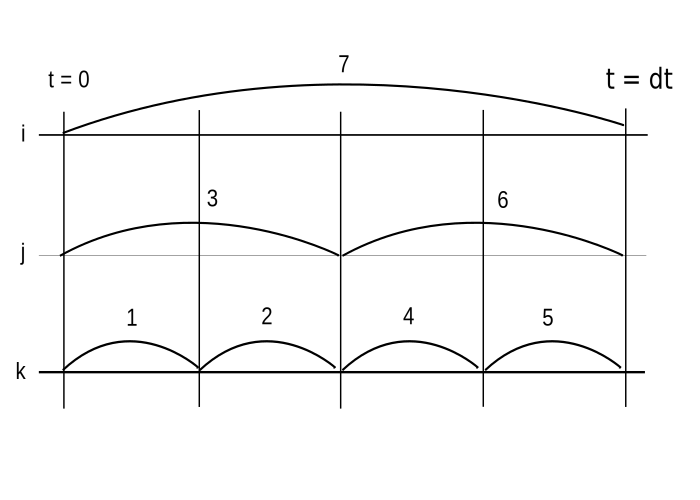
\includegraphics[width=12cm]{./figures/steps.png}
\caption{The order of updating the bodies i, j and k using the time steps $\dtm$, $\dtm/2$ and $\dtm/4$ respectively. The numbers above each arrow indicates the order of computations. At each pass of the integration loop, these steps are taken. At the end of each pass, the time steps of all the bodies are recomputed.}
\label{steps}
\end{center}
\end{figure}

A very important implementation detail when using this scheme is hidden away in the pseudocode statement \verb+update states of bodies using time step dt*+. We now explain how this step is taken. First, when updating the states of the bodies using the smallest time step we need to know the value of $a_{i+1}$ for these bodies. This in turn depends upon the positions of \emph{all} the bodies at this time step. We find these by extrapolating the positions of all the other planets to time $t + \dt_{\mathrm{min}}$. The bodies with larger time steps are simply moved the correct amount along their current \verb+v_half+ vector. These extrapolated positions are not added to the \verb+state_history+ of the bodies. When going on to compute new states for the bodies using time step $\dt_{\mathrm{med}}$, we can use the current (newly updated) positions of the planets using the smallest time step. The bodies using the largest time step still need to be extrapolated. This is done in the same manner, this time moving $\dt_{\mathrm{med}}$ steps along their \verb+v_half+. Now new states are added twice for the bodies using the medium time step, in order to stay synchronised in time with the other bodies. Finally when computing new states for the bodies using the largest time step we may use the current positions of all the other bodies along with extrapolated positions of the bodies themselves. New states are added four times for these bodies in order to stay synchronised in time. Although $a_{i+1}$ will always depend upon the positions of \emph{all} the planets at any given time, the function \verb+gravity(states)+ is written in such a way as only to return the gravitational acceleration on the bodies using the time step corresponding to the value of \verb+current_dt+.   

The implementation found in \verb+APNBodySolver+ has several weaknesses. A lot could be done to improve the speed of the integration loop as a lot of time is spent simply moving data around, and also several values are computed many times. In return the implementation is easy to understand and the basic idea of using adaptive time steps gets across. If I were to start over I would definitely omit object orientation of the bodies. This seems to me unnecessary encapsulation of data, and going over to a more purely matrix based implementation would have many benefits. Also allowing more time steps would definitely be worth spending some time on. This could be achieved by altering the algorithm presented above with more clever loops and use of modular arithmetic to synchronise and extrapolate nicely.

\subsection{Parallellization}

When it came to parallelising the code, we chose to do this using the OpenMP library. This proved to in principle be extremely simple, consisting only of one line of code; 

\begin{verbatim}
#pragma omp parallel for reduction(+:ax, ay, az) num_threads(threads)
\end{verbatim} 

The part of the program that is most suited for parallelisation is the brute force gravity computation (although other parts, such as recomputing time steps could also benefit from parallelisation). The function \verb+gravity(states)+ first iterates over all bodies with the correct time step. Once the central body is chosen, \verb+threads+ threads are spawned to iterate over all the other bodies in parallel and accumulate the components of the acceleration on the central body in the private variables \verb+ax+, \verb+ay+ and \verb+az+. Once all the threads have finished iterating, they \emph{reduce} the variables \verb+ax+, \verb+ay+ and \verb+az+ using the addition operator. This means that all the threads add their private acceleration components together so that in the end, \verb+ax+, \verb+ay+ and \verb+az+ contain the accelerations due to \emph{all} the other planets. The outer loop then goes on to the next body \&c. 

In practice however, it seems that something went wrong along the way. The results of the simulations are consistently good, but there is no speedup whatsoever due to parallelisation, on the contrary the simulations take longer the more threads are used as can be seen in fig. \ref{par}.

\begin{table}[htdp]
\caption{Time in seconds taken to solve the 100-, 250- and 1000 body systems using 1-4 threads.}
\begin{center}
\begin{tabular}{c|c|c|c|c}
$N$ & 1 & 2 & 3 & 4 \\
\hline
100 & 0.452672 & 1.035 & 1.19734 & 1.23063  \\
250 & 0.891804 & 1.80142 & 2.05254 & 2.14533 \\
1000 & 10.5088 & 11.7438 & 11.9723 & 11.6965 \\
\end{tabular}
\end{center}
\label{par}
\end{table}

\emph{That} is what should be called embaressingly parallel. Unfortunately, this problem has not been solved in the time of writing. Something will have to be done at a later time to fix the \verb+P+ part of \verb+APNBodySolver+.

\section{Refined results for the solar system}
 
Forgetting the broken parallelisation, the improved $N$-body solver reproduces the results of the inner solar system quite well, and does take shorter time, although it is quite tricky to directly compare the two solvers, as described earlier. 

\subsection{Animations}

As a fun application of the trajectories generated, a 3D animation of the inner solar system was implemented using the OpenGL library. The planets are modelled as textured spheres revolving around the sun. The relative sizes and rotation periods are not to scale, but the trajectories are accurate. The program can be found in \verb+source/OpenGL_solarsystem.cpp+ of the main project page. A executable compiled on a Macbook Pro running OSX 10.9.5 can also be found there. On other architectures the executable should be compileable by running \verb+make solar_animation+ in a terminal. We do not go into implementation details as the code should speak for itself. 

\begin{figure}[H]
\begin{center}
\includegraphics[width=12cm]{./figures/ISS_screenshot.png}
\caption{Screenshot of a run of solar\_animation. From left to right we see Earth, Venus, Mercury, Sun, Jupiter and Mars.}
\label{default}
\end{center}
\end{figure}

\begin{figure}[H]
\begin{center}
\includegraphics[width=12cm]{./figures/matlab_animation1}
\caption{Still images from Matlab-generated animations of three different subsystems of the inner solar systems.}
\label{default}
\end{center}
\end{figure}


\section{Further development of the algorithm}

As wee have seen, the final \verb+APNBodySolver+ is quite an advanced and capable solver. Before moving on to our final application of the solver we take a moment to consider what more could be done to improve the solver. 

\subsection{Faster gravity evaluations}

The brute-force method of computing the mutual gravitational attraction between $N$ bodies is a $\mathcal{O}(N^2)$ computation. However there are different ways around this costly computation. One of the more popular is the so-called Barnes-Hut tree-method. This way of computing gravitational attraction is of order $\mathcal{O}(N\log N)$. The method is very neat, and we give a summary of it here. At each gravity evaluation, the volume of integration is first subdivided into eight equal subcells. These subcells are then recursively subdivided until only one body is present in each cell. This gives rise to a oct-tree of subcells; starting at the root node consisting of the entire integration volume, each descendent will either be a cell containing many bodies and eight descendants of its own, or it will be a cell containing only one body. This tree has to be generated at each gravity evaluation. To compute the gravitational attraction on a body, the tree is traversed from the root node, and if the centre of mass of any other cell is far enough away from the body in question, all the bodies in this cell are considered as one particle located at the centre of mass of this cell. By changing what is meant by 'far enough', the accuracy of the computation varies. If 'far enough' is set to infinity, the algorithm collapses into the brute force evaluation. For more on the Barnes-Hut tree code, see \cite{barneshut} 

\subsection{Smoothing factor}

When simulating large $N$ systems, it often occurs that two or more bodies move arbitrarily close to each other. Thus we often experience the singularity at $r_{ij} = 0$ in \eqref{gravity}. This is both physically and numerically a undesirable effect, that can easily be cured. Physically, because in most cases we are not interested in point-masses, but rather distributions of mass in space. In fact a 'body' in a simulation could be understood to represent several stars and interstellar dust in some cases. So there are several physical reasons to remove the singularity. Numerically it is undesirable because the acceleration on the bodies becomes so large that the time step needs to be drastically reduced in order to retain a stable solution. There are several ways of removing the singularity, one particularly simple method is perturbing Newtons' equation slightly to read

\begin{equation}
a_i = \sum_{j\neq i}\frac{G m_j}{r_{ij}^2 + \epsilon^2}\i_{ij}
\end{equation}

This modification is actually implemented in \verb+APNBodySolver+, and the value of $\epsilon$ can be given as input to the solver (typically a small number). We study the effect of varying $\epsilon$ in the final section. 

\section{Application: open cluster collapse}

\subsection{Introduction}

In this final section we will use the $N$-body solver developed in the preceding sections to study a toy model of a small cluster of stars. The system initially consists of $N$ bodies at rest uniformly distributed within a sphere of radius of $R_0 = 20$ light years. The masses of the bodies are taken from a normal distribution with mean mass 10 $M_{\odot}$ and standard deviation $1M_{\odot}$. This is an appropriate model for studying so-called \emph{open clusters}. An open cluster is a group of up to a few thousand stars that were formed from the same giant molecular cloud and have roughly the same age. More than 1100 open clusters have been discovered within the Milky Way Galaxy, and many more are thought to exist. They are loosely bound to each other by mutual gravitational attraction and become disrupted by close encounters with other clusters and clouds of gas as they orbit the galactic center, resulting in a migration to the main body of the galaxy as well as a loss of cluster members through internal close encounters. Open clusters generally survive for a few hundred million years, with the most massive ones surviving for a few billion years \cite{wikicluster}.

\begin{figure}[H]
\begin{center}
\includegraphics[width=8cm]{./figures/wikicluster}
\caption{NGC 265, an open star cluster in the Small Magellanic Cloud}
\label{wikicluster}
\end{center}
\end{figure}

Before we delve into the results, lets consider some theoretical aspects of our open cluster model. A excellent paper on the subject can be found here \cite{opencluster}, and we refer the specially interested reader thither for a more detailed and sound discussion. The selection of results found in the next section is largely inspired by that paper. 

In the limit as $N\to\infty$ keeping the initial density constant we get a continuous fluid. In this case, the system collapses into a singularity at a finite time $\tc = \sqrt{\frac{3\pi}{32G\rho_0}}$, where $\rho_0$ is the mass density in the initial integration volume. In all the simulations we use units of solar masses, light years and $\tc$. As we saw in \eqref{scaleG} this determines the value of $G^*$ (the scaled value of $G$).

\begin{equation}
G^* = \frac{G m^* {t^*}^2}{{r^*}^3} = \frac{G M_{\odot}\tc^2}{1ly^3}
\label{gscale}
\end{equation} 

Inserting

\begin{equation}
\rho_0 = \frac{N10M_{\odot}}{\frac{4\pi R_0^3}{3}}
\end{equation}

into the expression for $\tc$ yields

\begin{equation}
\tc^2 = \frac{\pi^2 R_0^3}{8GN10M_{\odot}}
\end{equation}

and inserting this again in \eqref{gscale} yields

\begin{equation}
G^* = \frac{GM_{\odot}\pi^2 20^3 ly^3}{8 GN 10 M_{\odot} ly^3} = \frac{100\pi^2}{N}.
\end{equation}

This is the value of $G$ used in the simulations. 

\subsection{Results}

We now present the results obtained using the solvers presented earlier. The following properties were stored for analysis in each run; trajectories, total mechanical energy, virial energy of bound bodies, number of bound bodies, time taken by simulation, $\dtm$ and $\epsilon$. We use as test cases $N = 100, 250, 1000$, fixing $T = 6\tc$, and studying the results as we vary $\epsilon$ and $\eta$.  

Visually the results were quite similar throughout the simulations, and also consistent with known physical and astronomical facts about open clusters. After roughly one unit of time the system collapses into a much smaller sphere than initially. Then the system 'explodes' outwards, ejecting several particles and leaving behind a rather closely bound center with a larger, less dense halo enveloping the core. Since the results all 'look' good, we need to use different methods to evaluate the accuracy of the simulations. This we can do by looking at the total mechanical energy of the entire system. Theoretically, since this is a closed system, it is a conserved quantity. A simple test is therefore to see to which extent energy is conserved.

\begin{figure}[H]
\begin{center}
\includegraphics[width=12cm]{./figures/clusterenergy1}
\caption{Total mechanical energy of open cluster integrated over a period of 6$\tc$ for $\epsilon = 0.1$ and $\epsilon = 0.01$. The solver chose maximum time steps 0.0026, 0.00431 and 0.00438 for the 100-, 250-, 1000-body systems respectively.}
\label{clusterenergy1}
\end{center}
\end{figure}

As wee see in fig. \ref{clusterenergy1}, the degree to which energy is conserved depends greatly upon the value of $\epsilon$. The difference can easily be seen in the animations, with close encounters being much more prominent in low $\epsilon$ simulations. It can be inferred from the energy plot that choosing $\epsilon$ too low is not a good choice energy-wise. It seems that when an encounter is very close, and the smoothing factor is not chosen large enough, the bodies are flung away from each other, increasing their energy by a large amount. This explains the tendency for the energy to drift linearly when $\epsilon$ is too small. This is typical behaviour for Verlet-style integration schemes. Also we note that the drift is much more prominent as $N$ increases, perhaps because the number of close encounters increases as well. On the other hand, one could ask when $\epsilon$ is too large. Close encounters \emph{are} often important in open cluster dynamics, and choosing $\epsilon$ too large will force the system to act unphysically. We leave the question open-ended, and refer to \cite{smoothing} for a discussion of some technicalities of choosing $\epsilon$. 

Another way of testing the accuracy of the solver is to test the virial theorem. The virial theorem states that for any bound gravitational system in equilibrium we have

\begin{equation}
2 \langle K \rangle = -\langle V\rangle,
\label{virial}
\end{equation}

where $\langle K \rangle$ is the time-average kinetic energy, and $\langle V\rangle$ is the time-average potential energy. By the ergodic hypothesis we can take an ensemble average over all bound bodies rather than time-average. By \emph{bound} body, we mean a body with negative energy. A bound body does not have enough energy to escape from the cluster. The virial theorem only applies to the bound bodies. In the function \verb+writeEnergy()+, the quantity $2 \langle K \rangle + \langle V\rangle$ is computed at each time-step after first determining which of the bodies are in fact bound. Ideally, this quantity should be close to zero after the system reaches equilibrium. The results can be found in fig. \ref{virial1}.

\begin{figure}[H]
\begin{center}
\includegraphics[width=12cm]{./figures/clustervirial1}
\caption{Virial energy of bound bodies in open cluster integrated over a period of 6$\tc$. The solver chose maximum time steps 0.026, 0.0431 and 0.438 for the 100-, 250-, 1000-body systems respectively.}
\label{virial1}
\end{center}
\end{figure}

We see that after the system has reached equilibrium the quantity $2 \langle K \rangle + \langle V\rangle$ fluctuates around 0. This fluctuation is completely fine since the virial theorem is a statistical statement. The fact that the virial energy consistently has a bias toward negative values is a bit more worrying. We also see a slight trend for the virial energy to be lower as $N$ increases. It is again tempting to draw the conclusion that too much 'free kinetic energy' is gained through close encounters during the collapse, and that after the collapse the system has increased its energy. This argument seems tempting, but in the case of $\epsilon = 0.1$, it is also inconsistent with the (conserved) total energy seen in fig. \ref{clusterenergy1}.

Let us before we consider this question in more detail take a look at the evolution of the number of bound bodies. As mentioned, we say that a body is bound if it has positive energy. In fig. \ref{bound1}, we see how the number of bound bodies depends upon $\epsilon$ and $N$. 

\begin{figure}[H]
\begin{center}
\includegraphics[width=12cm]{./figures/clusterbound1}
\caption{Fraction of bound bodies in 100-, 250- and 1000-body simulation.}
\label{bound1}
\end{center}
\end{figure}

To begin with, all bodies are of course bound. Then follows a period of contraction, where many of the bodies pick up a lot of kinetic energy and become unbound. After the system reaches its smallest radius follows a period of 'explosion', here the number of bound bodies increases. After equilibrium is reached the fraction seems to stay relatively constant. As $N$ increases, the fraction of bound bodies in the equilibrium state also increases. Perhaps this is because there is simply \emph{more} mass in the initial sphere for larger $N$. Therefore the cluster is more tightly bound by the presence of more gravitational 'sinks'. Once again the effect of altering $\epsilon$ becomes clear when we compare the left and right plots in fig. \ref{bound1}. With a lower value of $\epsilon$ the cluster is less tightly bound, and therefore only 50\%-75\% of the bodies remain bound in equilibrium for $\epsilon = 0.01$, whilst for $\epsilon = 0.1$, roughly 70\%-90\% remain bound. Another way of observing this property of $\epsilon$ would be to plot the smallest radius attained by the system (at $\tc$), as a function of $\epsilon$. We hypothesise that this radius should in some way be proportional to $\epsilon$. A lot more on this can be found in \cite{smoothing}.

To complete the picture we plot the boundedness results of a longer simulation ($T = 15\tc$). 

\begin{figure}[H]
\begin{center}
\includegraphics[width=12cm]{./figures/longbound}
\caption{Fraction of bound bodies in 250-body system integrated for a longer period.}
\label{bound2}
\end{center}
\end{figure}

With a longer time scope several new features emerge. It seems that for $\epsilon= 0.1$, the equilibrium state is in fact stable, i.e.. bodies are not ejected after equilibrium is reached with around 85\% of the bodies remaining bound. But in the case of $\epsilon = 0.01$, it seems that bodies are being ejected at a steady rate long after 'equilibrium' is reached. Which one of the two pictures is correct is not answerable with the information at hand. Though energy considerations led us to believe $\epsilon = 0.1$ is a good value there are several reasons why this is too large. 

\subsection{Graphics}

In this section also, OpenGL animations were generated. The program can be found in \verb+openGL_cluster.cpp+. We present some screenshots from the animations. 

\begin{figure}[H]
\begin{center}
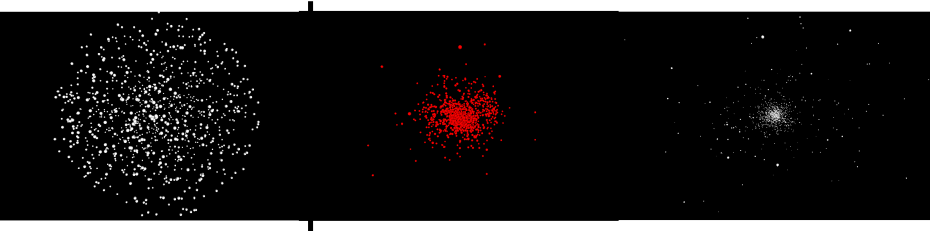
\includegraphics[width=14cm]{./figures/cluster1000}
\caption{Screenshots from OpenGL animation of 1000-body cluster. On the left we have the initial conditions, in the middle we see the system after one $\tc$ and on the right we have the cluster in its equilibrium state at $t=6\tc$. It is interesting to note the similarity of the righmost picture with fig. \ref{wikicluster}}
\label{default}
\end{center}
\end{figure}

\begin{figure}[H]
\begin{center}
\includegraphics[width=10cm]{./figures/structure}
\caption{A interesting 1000-body simulation where we can see very clearly the formation of two distinct cores. This structure formation is not at all unexpected, and is most probably caused by small density fluctuations in the initial conditions. These small deviations from spherical symmetry are accentuated after the system has interacted for a substantial period of time. Gravity is a truly awesome force, being the creator of structure on length scales from sand-castles to universes.}
\label{default}
\end{center}
\end{figure}

\section{Conclusion}

The goal of this project was to learn as much as possible about computational physics. I conclude that I have been completely successfull in achieving this. I have learned a lot about C++, using makefiles, managing the structure of a large project, writing a scientific report, dimentional analysis, numerical integration, using third party libraries, using OpenGL and OpenMP and much more. When it comes to the actual results on the other hand, I can not say I am entirely happy. In any numerical simulation of a physical system there will always be the question, 'to which degree can we trust the results?'. For most of the results in this paper, the answer is 'probably not very much'. It would be better if I at least had run sufficiently rigorous tests to say 'certainly not very much'. The presentation in this paper is more of a show-and-tell presentation than the accurate, tested, peer-reviewable format appropriate in a scientific paper. So I have even learned a lot from the many mistakes made during the writing of this project, with perhaps the most valuable lesson being to work in a team next time. 

\section*{Aknowledgments}

Many thanks to Morten Hjort-Jensen, H�vard Tveit Ihle, Andreas Hafreager and Morten Ledum for guidance along the way. 

%====================BIBLIOGRAPHY===========================
\begin{thebibliography}{9}

\bibitem{github}
	http://github.com/gudbrandtandberg/N-Body

\bibitem{adaptive}
	'A Time-Symmetric Block Time-Step Algorithm for N-Body Simulations'\\
	Junichrio Makino, Piet Hut, Murat Kaplan, Hasan Saygin\\
	\emph{New Astron.} 12 (2006) 124-133

\bibitem{barneshut}
	'A hierarchical O(N logN) force-calculation algorithm'\\
	Josh Barnes \& Piet Hut\\
	\emph{Nature} vol. 324 
	
\bibitem{opencluster}
	'Cold uniform spherical collapse revisited' \\
	M. Joyce, B. Marcos and F. Sylos Labini\\
	\emph{Astro-ph.} 2 Nov 2010

\bibitem{wikicluster}
	http://en.wikipedia.org/wiki/Open\_cluster

\bibitem{aarseth}
	'Gravitational N-body Simulations: Tools and Algorithms' \\
	Sverre Aarseth\\
	\emph{Cambridge Monographs on Mathematical Physics}

\bibitem{smoothing}
'Gravitational softening as a smoothing operation'\\
Joshua E. Barnes \\
\emph{Mon. Not. Astrom. Soc.} Aug 2012
\end{thebibliography}


\end{document}  